% 1984 年全国卷（文科）第 15 题：正三棱柱（底面三角形 A 在前、B 在右、C 在左，三条侧棱竖直），
% 经过底面一边 AB 作与底面成 30° 角的平面，截面为三角形 ABD，D 在过 C 的侧棱上；
% 顶面可见，故顶面三边画实线；底面后边 CB 与被后侧面遮住的截面边 DB 画虚线（按源卷布局）
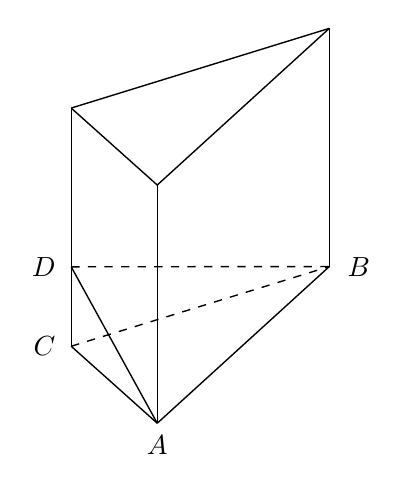
\begin{tikzpicture}[scale=1.15, line width=0.5pt,
  every node/.style={inner sep=1.5pt}]
  % 顶点坐标（按源卷布局手算：底面三顶点 + 各自正上方等高 H=2.63 的顶面三顶点）
  \coordinate (A)  at (0.95, 0);      % 底面前顶点
  \coordinate (B)  at (2.85, 1.73);   % 底面右顶点
  \coordinate (C)  at (0.00, 0.85);   % 底面左顶点
  \coordinate (A1) at (0.95, 2.63);   % 顶面前顶点（在 A 正上方）
  \coordinate (B1) at (2.85, 4.36);   % 顶面右顶点（在 B 正上方）
  \coordinate (C1) at (0.00, 3.48);   % 顶面左顶点（在 C 正上方）
  \coordinate (D)  at (0.00, 1.727);  % 侧棱 CC1 上一点，C 到 D 约为 C 到 C1 的 1/3
  % 被遮住的棱：底面后边 CB、截面边 DB
  \draw[dashed] (C) -- (B);
  \draw[dashed] (D) -- (B);
  % 可见的棱
  \draw (A) -- (B);
  \draw (A) -- (C);
  \draw (A) -- (A1);
  \draw (B) -- (B1);
  \draw (C) -- (C1);
  \draw (A1) -- (B1);
  \draw (A1) -- (C1);
  \draw (C1) -- (B1);
  % 截面三角形 ABD 在可见侧面 ACC1A1 内的边 AD
  \draw (A) -- (D);
  % 标注
  \node[anchor=north] at (0.95,-0.08) {$A$};
  \node[anchor=west] at (3.00,1.73) {$B$};
  \node[anchor=east] at (-0.12,0.85) {$C$};
  \node[anchor=east] at (-0.12,1.727) {$D$};
\end{tikzpicture}
